\subsection{Videooptagelser}
\label{VideooptagelserValgAfGestikker}
%
I følgende afsnit vil de visuelle repræsentationer af de udvalgt gestikker blive udarbejdet. Der udarbejdes tre videoer; én hvor de udvalgte semaforiske gestikker til pause og start fremgår, én hvor de udvalgte semaforiske gestikke til at skifte musiknummer frem og tilbage fremgår og én hvor de udvalgte semaforiske gestikker til at skrue op og ned for musikken fremgår. Videooptagelserne redigeres i Windows Movie Maker version 2012 og de tre færdigredigerede videooptagelser fremgår i \textbf{elektroniske bilag}. 
\blankline
%
Fælles for de tre videooptagelser er, at de er optaget med et Canon Powershot s110 kamera på et stativ, kameraet optager både billede og lyd, optagelserne er taget med en 45$^{\circ}$'s vinkel i et halvnært perspektiv samt en neutral hvid baggrund og et neutralt ansigtsudtryk, hvilket er illustreret på \autoref{fig:Tryk}. Ved at optage med en 45$^{\circ}$'s vinkel i et halvnært perspektiv er det muligt at tydeliggøre størrelse, bevægelsesretning og dybde for hver af de udvalgte semaforiske gestikker. Ydermere tillader en 45$^{\circ}$'s vinkel at forstyrrelser i form af øjenkontakt mellem testperson og demonstratoren i optagelserne, minimeres. 
%
\begin{figure}[H]
	\centering
	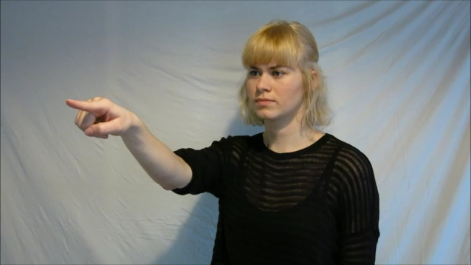
\includegraphics[resolution=300,width=\textwidth]{Flowdiagram/Tryk}
	\caption{Illustration af hvordan optagelserne foretages, med 45$^{\circ}$'s vinkel i et halvnært perspektiv samt en neutral hvid baggrund og et neutralt ansigtsudtryk.}
	\label{fig:Tryk}
\end{figure}
\noindent
%
Under optagelserne afspilles der musik fra en computer. Musiknummeret til at pause og starte musikken er \enquote{Stay} fra Zedd og Alessia Cara (2017). Musiknumrene til at skifte sang frem og tilbage er \enquote{Closer} fra The Chainsmokers ft. Halsey (2016) og \enquote{Galway Girl} fra Ed Sheeran (2017). Musiknummeret til at skrue op og ned for musikken er \enquote{You Don't Know Me} fra Jax Jones ft. RAYE (2017). Når der eksempelvis laves en gestik for at pause musikken, pauses musikken på computeren, for på den måde at demonstrerer hvilken gestik, der skal til for at musikken pauses. De resterende funktioner optages på tilsvarende måde.\blankline
%
Når de udvalgte semaforiske gestikker er blevet optaget, bliver de som tidligere nævnt redigeret i Windows Movie Maker version 2012. På \autoref{fig:FlowdiagramPause} illustreres rækkefølgen på de skærmbilleder, som videoerne består af. Eksemplet på \autoref{fig:FlowdiagramPause} er videoen der gengiver de udvalgte semaforiske gestikker til at pause og starte musikken, de to andre videoer er bygget op omkring den samme struktur, dog indeholder videoen for at skrue op og ned for musikken ydereligere fire skærmbilleder, hvor to angiver hvilket gestik-par nummer der præsenteres og to gengiver gestik-parret.       
%
\begin{figure}[H]
	\centering
	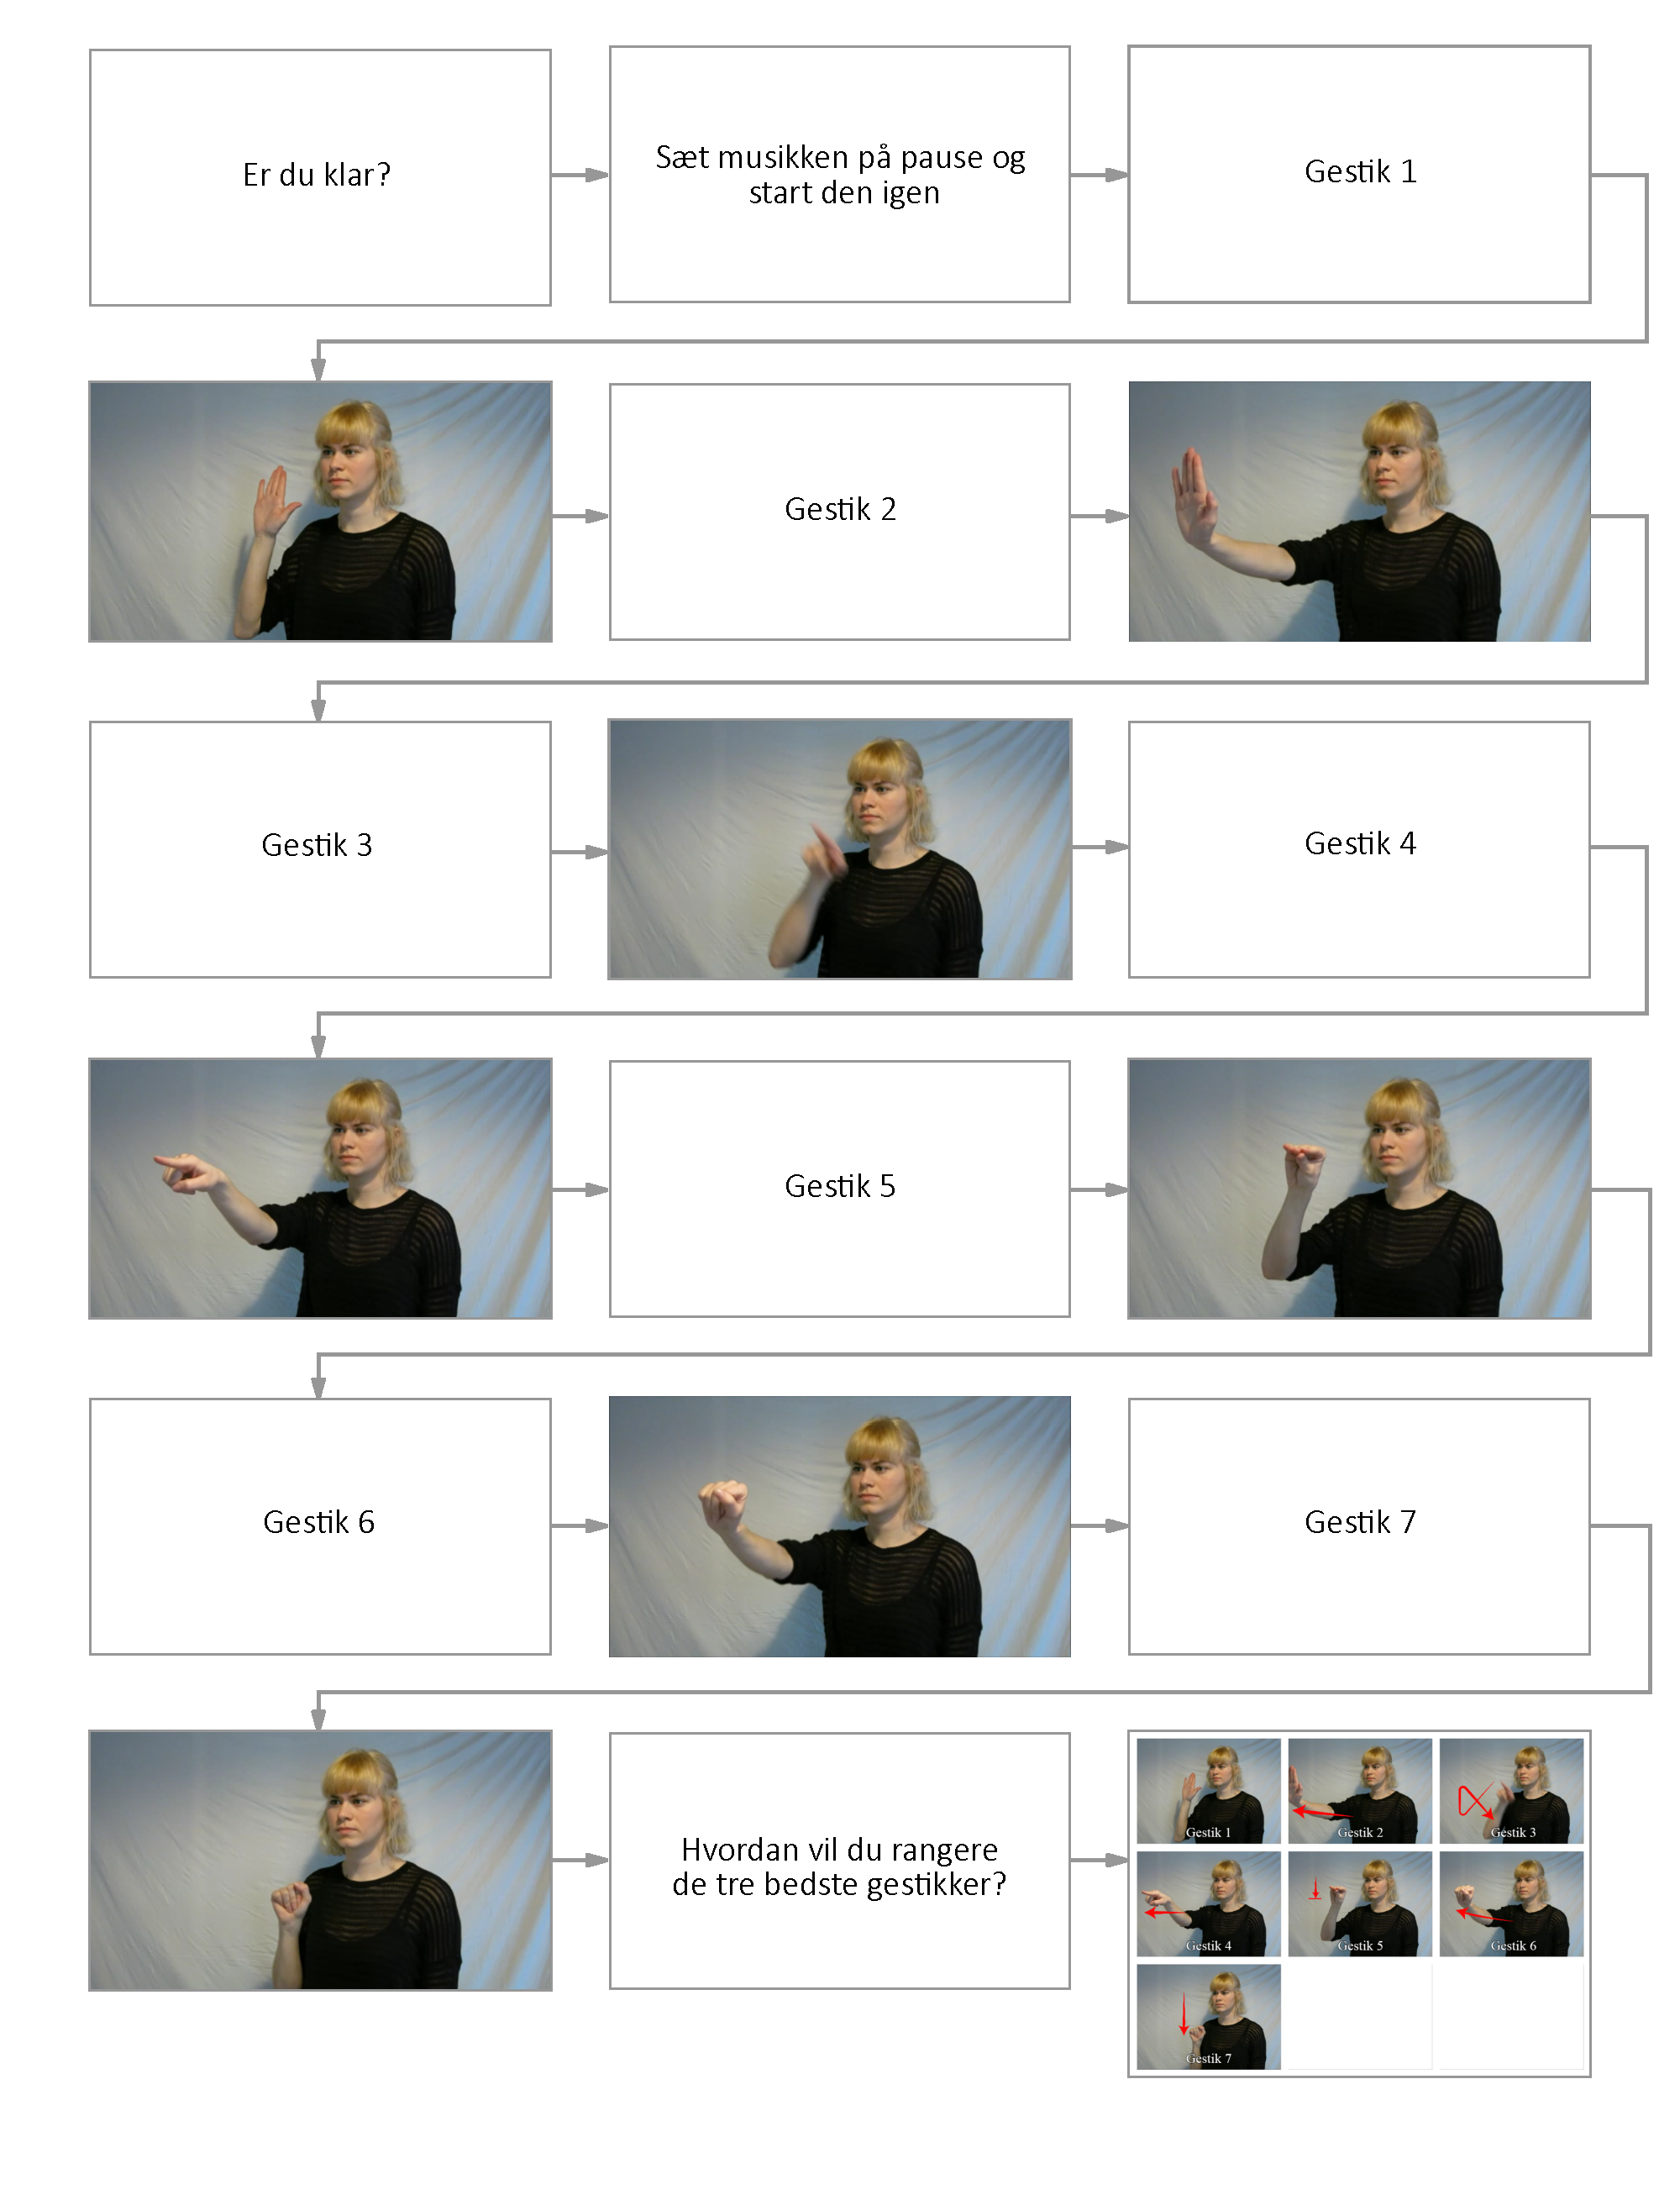
\includegraphics[resolution=300,width=\textwidth]{Flowdiagram/FlowdiagramPauseogStart}
	\caption{Illustration af hvilke skærmbilleder, der indgår i videoen til at pause og starte musikken. De to resterende videoer er bygget op omkring den samme struktur.}
	\label{fig:FlowdiagramPause}
\end{figure}
\noindent
%
Det første skærmbillede testpersonerne præsenteres for består af teksten: \textit{Er du klar?} og præsenteres i to sekunder, før skærmbilledet med teksten: \textit{Sæt musikken på pause og start den igen} præsenteres i tre sekunder. Teksten på det andet skærmbillede tilpasses afhængigt af hvilken video, der afspilles men varigheden er fast. De nummerede skærmbilleder, eksempelvis med teksten: \textit{Gestik 1}, præsenteres alle med en to sekunders varighed. Det andet sidst skærmbillede med teksten: \textit{Hvordan vil du rangere de tre bedste gestikker?} præsenteres med fire sekunders varighed, før skærmbilledet med opsummeringen af de udvalgte gestikker præsenteres. Opsummeringen angives med en 30 sekunders varighed, da dette er den maksimale varighed i Windows Movie Maker version 2012, dog forsvinder skærmbilledet ikke efter de 30 sekunder. Det skal understreges at videoerne ikke indeholder statiske skærmbilleder af gestikkerne, da de er dynamiske og hvert gestik-par indeholder en modpart, som i dette tilfælde er at starte musikken, hvilket ikke er illustreret på \autoref{fig:FlowdiagramPause}.\blankline
%
Som illustreret på \autoref{fig:FlowdiagramPause} indeholder videoerne et skærmbillede hvor de udvalgte semaforiske gestikker opsummeres. På disse skærmbilleder er bevægelsen i gestikkerne forsøgt gengivet med retningspile, som er til for at testpersonerne kan adskille gestikkerne fra hinanden så de ikke behøver at huske gestikkerne, som de efterhånden introduceres i videoen. Derudover vil testpersonerne få mulighed for at få genspillet videoen, hvis de ønsker. Ydermere er gestikkerne nummerede afhængigt af den rækkefølge de er blevet optaget i samt rækkefølgen de bliver præsenteret i for testpersonerne. På \autoref{fig:OversigtPauseStart} gengives opsummeringsskærmbilledet for at pause og starte musikken, igen er det kun pause-gestikken, der indgår i opsummeringen. Modparten blev beskrevet i \autoref{tab:IndsamledeGestikkerPause}.  
%
\begin{figure}[H]
	\centering
	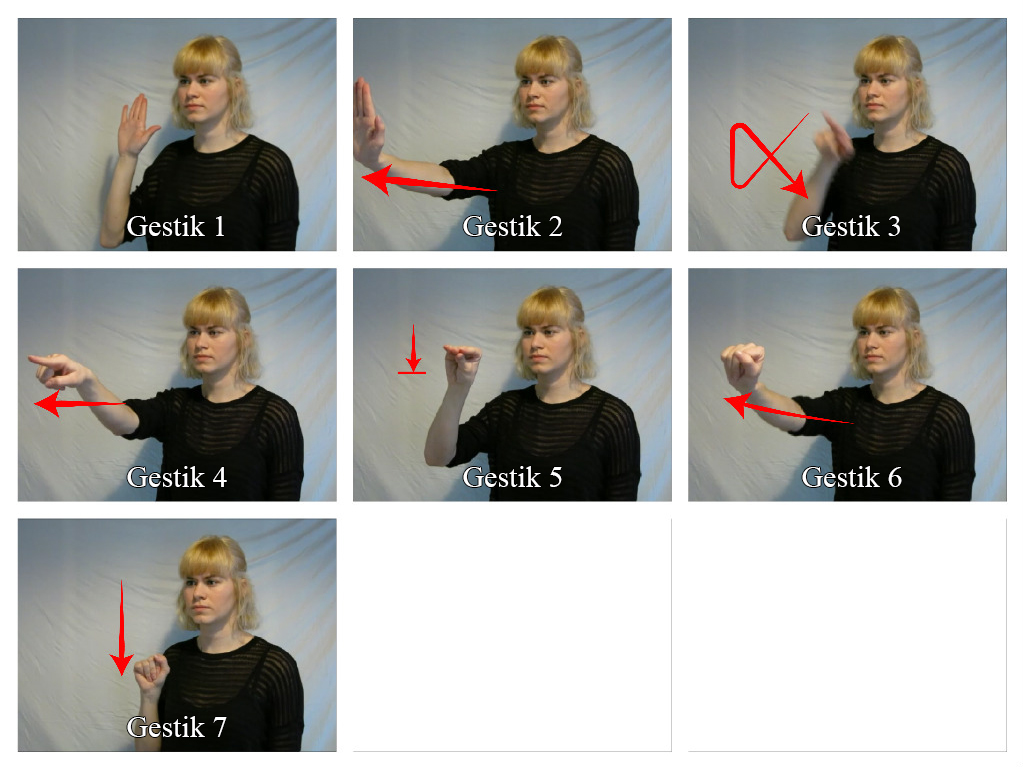
\includegraphics[resolution=300,width=\textwidth]{Test1/collage_start_pause_tekst}
	\caption{Opsummering af de syv semaforiske gestikker, der pauser og starter musikken, inklusiv nummerering og pile, som indikerer bevægelsesretning.}
	\label{fig:OversigtPauseStart}
\end{figure}
\noindent
%
Ligesom illustreret på \autoref{fig:OversigtPauseStart} gengives de udvalgte semaforiske gestikker til at skifte musiknummer frem og tilbage ligeledes med retningspile, for at indikere bevægelsen ved hver gestik, jævnfør \autoref{fig:OversigtSkift}. Ydermere er gestikkerne på \autoref{fig:OversigtSkift} ligeledes nummeret efter samme princip, som ved at pause og starte musikken. Gestikkerne som illustreres på \autoref{fig:OversigtSkift} gengiver alle at der skiftes til det næste musiknummer, hvor modparten enten vil være den samme bevægelse den modsatte retning eller et peg i den modsatte retning af hvad der er angivet på \autoref{fig:OversigtSkift}. Modparten blev beskrevet i \autoref{tab:IndsamledeGestikkerSkift}.
%
\begin{figure}[H]
	\centering
	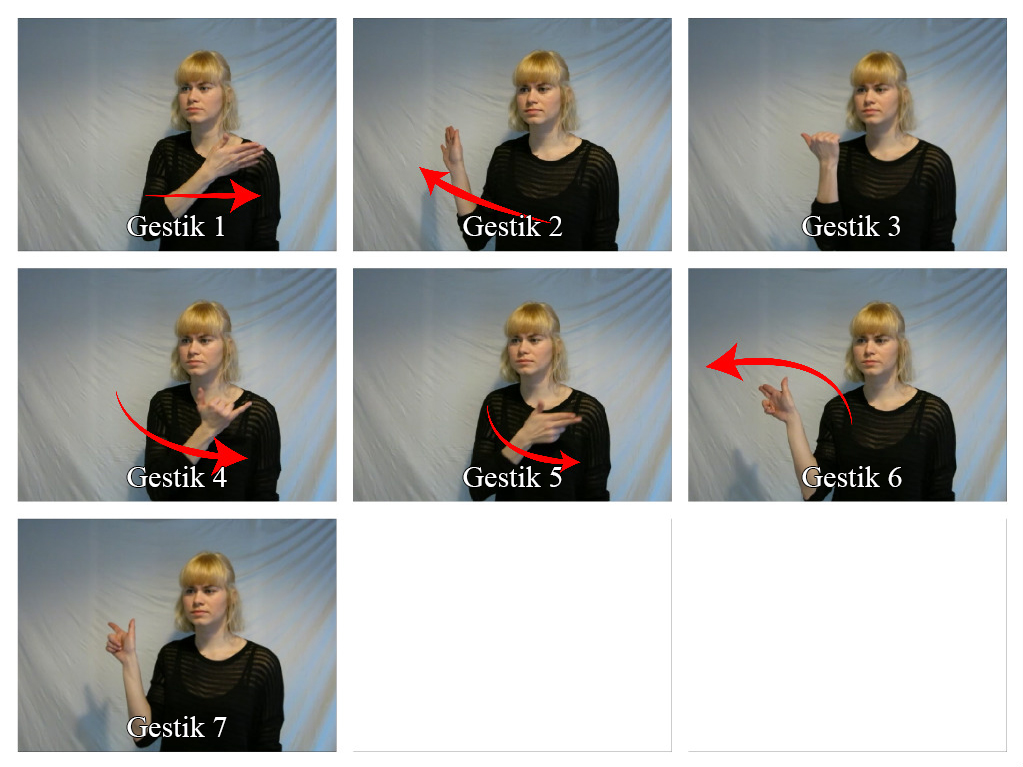
\includegraphics[resolution=300,width=\textwidth]{Test1/collage_Skiftsang_tekst}
	\caption{Opsummering af de syv semaforiske gestikker, der skifter musiknummer frem og tilbage, fra videoen, inklusiv nummerering og pile, som indikerer bevægelsesretning.}
	\label{fig:OversigtSkift}
\end{figure}
\noindent
%
Da både videoer og opsummeringsskærmbilleder er redigeret efter samme struktur, gengiver \autoref{fig:OversigtVolumen}, efter samme principper, opsummeringsskærmbilledet for at skrue op og ned for musikken.  
%
\begin{figure}[H]
	\centering
	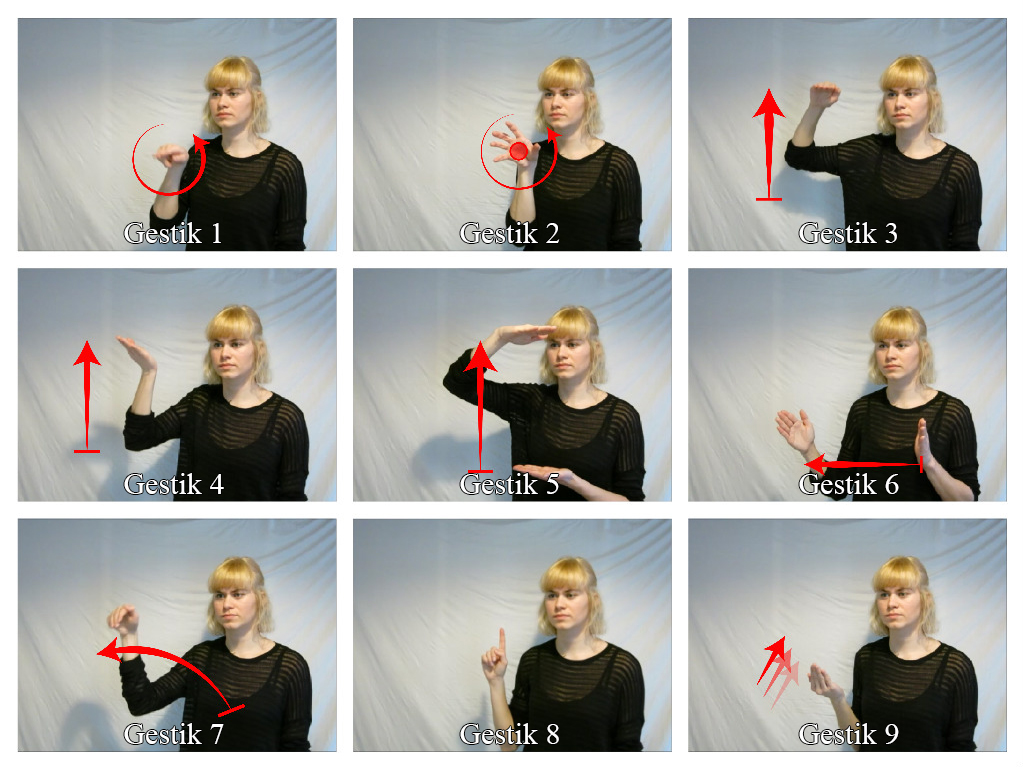
\includegraphics[resolution=300,width=\textwidth]{Test1/collage_volumen_tekst}
	\caption{Opsummering af de ni semaforiske gestikker til at skrue op og ned for musikken, fra videoen, inklusiv nummerering og pile, som indikerer bevægelsesretning.}
	\label{fig:OversigtVolumen}
\end{figure}
\noindent
%
Da der nu er udvalgt hvilke semaforiske gestikker, som potentielt kan knyttes til de seks funktioner i et musikanlæg samt udarbejdet tre videooptagelser, vil fokus i det følgende afsnit være rettet mod hvordan testen skal afvikles. 
